\documentclass{article}

% Packages for better formatting and math support
\usepackage{amsmath}
\usepackage{graphicx}
\usepackage{hyperref}
\usepackage{listings}
\usepackage{geometry}

% Adjust margins
\geometry{margin=0.8in}

% Title information
\title{CS456 Assignment 1: Section 3 Answers}
\author{Jiaze Xiao}
\date{\today}

\begin{document}

\maketitle

\section*{Question 1}
\begin{quote}
    How many TCP segments and UDP packets respectively are in \texttt{sample\_trace.pcapng}?
\end{quote}

\textbf{Answer:}
\begin{quote}
    TCP: 36 (frame 1-16 and 19-38)\\
    UDP: 2 (frame 17 and 18)
\end{quote}

\section*{Question 2}
\begin{quote}
    What is the destination port number of the UDP packet sent by the \textbf{client}?
\end{quote}

\textbf{Answer:}
\begin{quote}
    46025, the first UDP packet represents the start of negotiation from client (the \texttt{UPLOAD} request).
\end{quote}

\section*{Question 3}
\begin{quote}
    What is the destination port number of the UDP packet sent by the \textbf{server}?
\end{quote}

\textbf{Answer:}
\begin{quote}
    55746, the second UDP packet contains the \texttt{<r\_port>} sent back to the client from server.
\end{quote}

\section*{Question 4}
\begin{quote}
    Inspect the UDP packet sent by the \textbf{server}. What is the value of \texttt{r\_port} in this transfer? How did you find it?
\end{quote}

\textbf{Answer:}
\begin{quote}
    39351, the 4-byte data carried by the second UDP packet is \texttt{"00:00:99:b7"} and get 39351 after converting it from hex to decimal.
\end{quote}

\section*{Question 5}
\begin{quote}
    Identify the packet/segment which contained the contents of the transferred JSON file. What is its timestamp value (TSVal)? What is its length?
\end{quote}

\textbf{Answer:}
\begin{quote}
    Frame 22, TSVal: 2807180054, Length: 16491
\end{quote}

\section*{Question 6}
\begin{quote}
    Use the display filter to remove the packets that are not part of the communication between the client and server programs. What display filter did you use? Attach an image of the Wireshark window after the display filter has been applied.
\end{quote}

\textbf{Answer:}
\begin{quote}
    Using filter \texttt{frame.time\_relative > 15 \&\& frame.time\_relative < 16}\\
    (Or \texttt{frame.number >= 17 and frame.number <= 28} alternatively)
    \begin{center}
        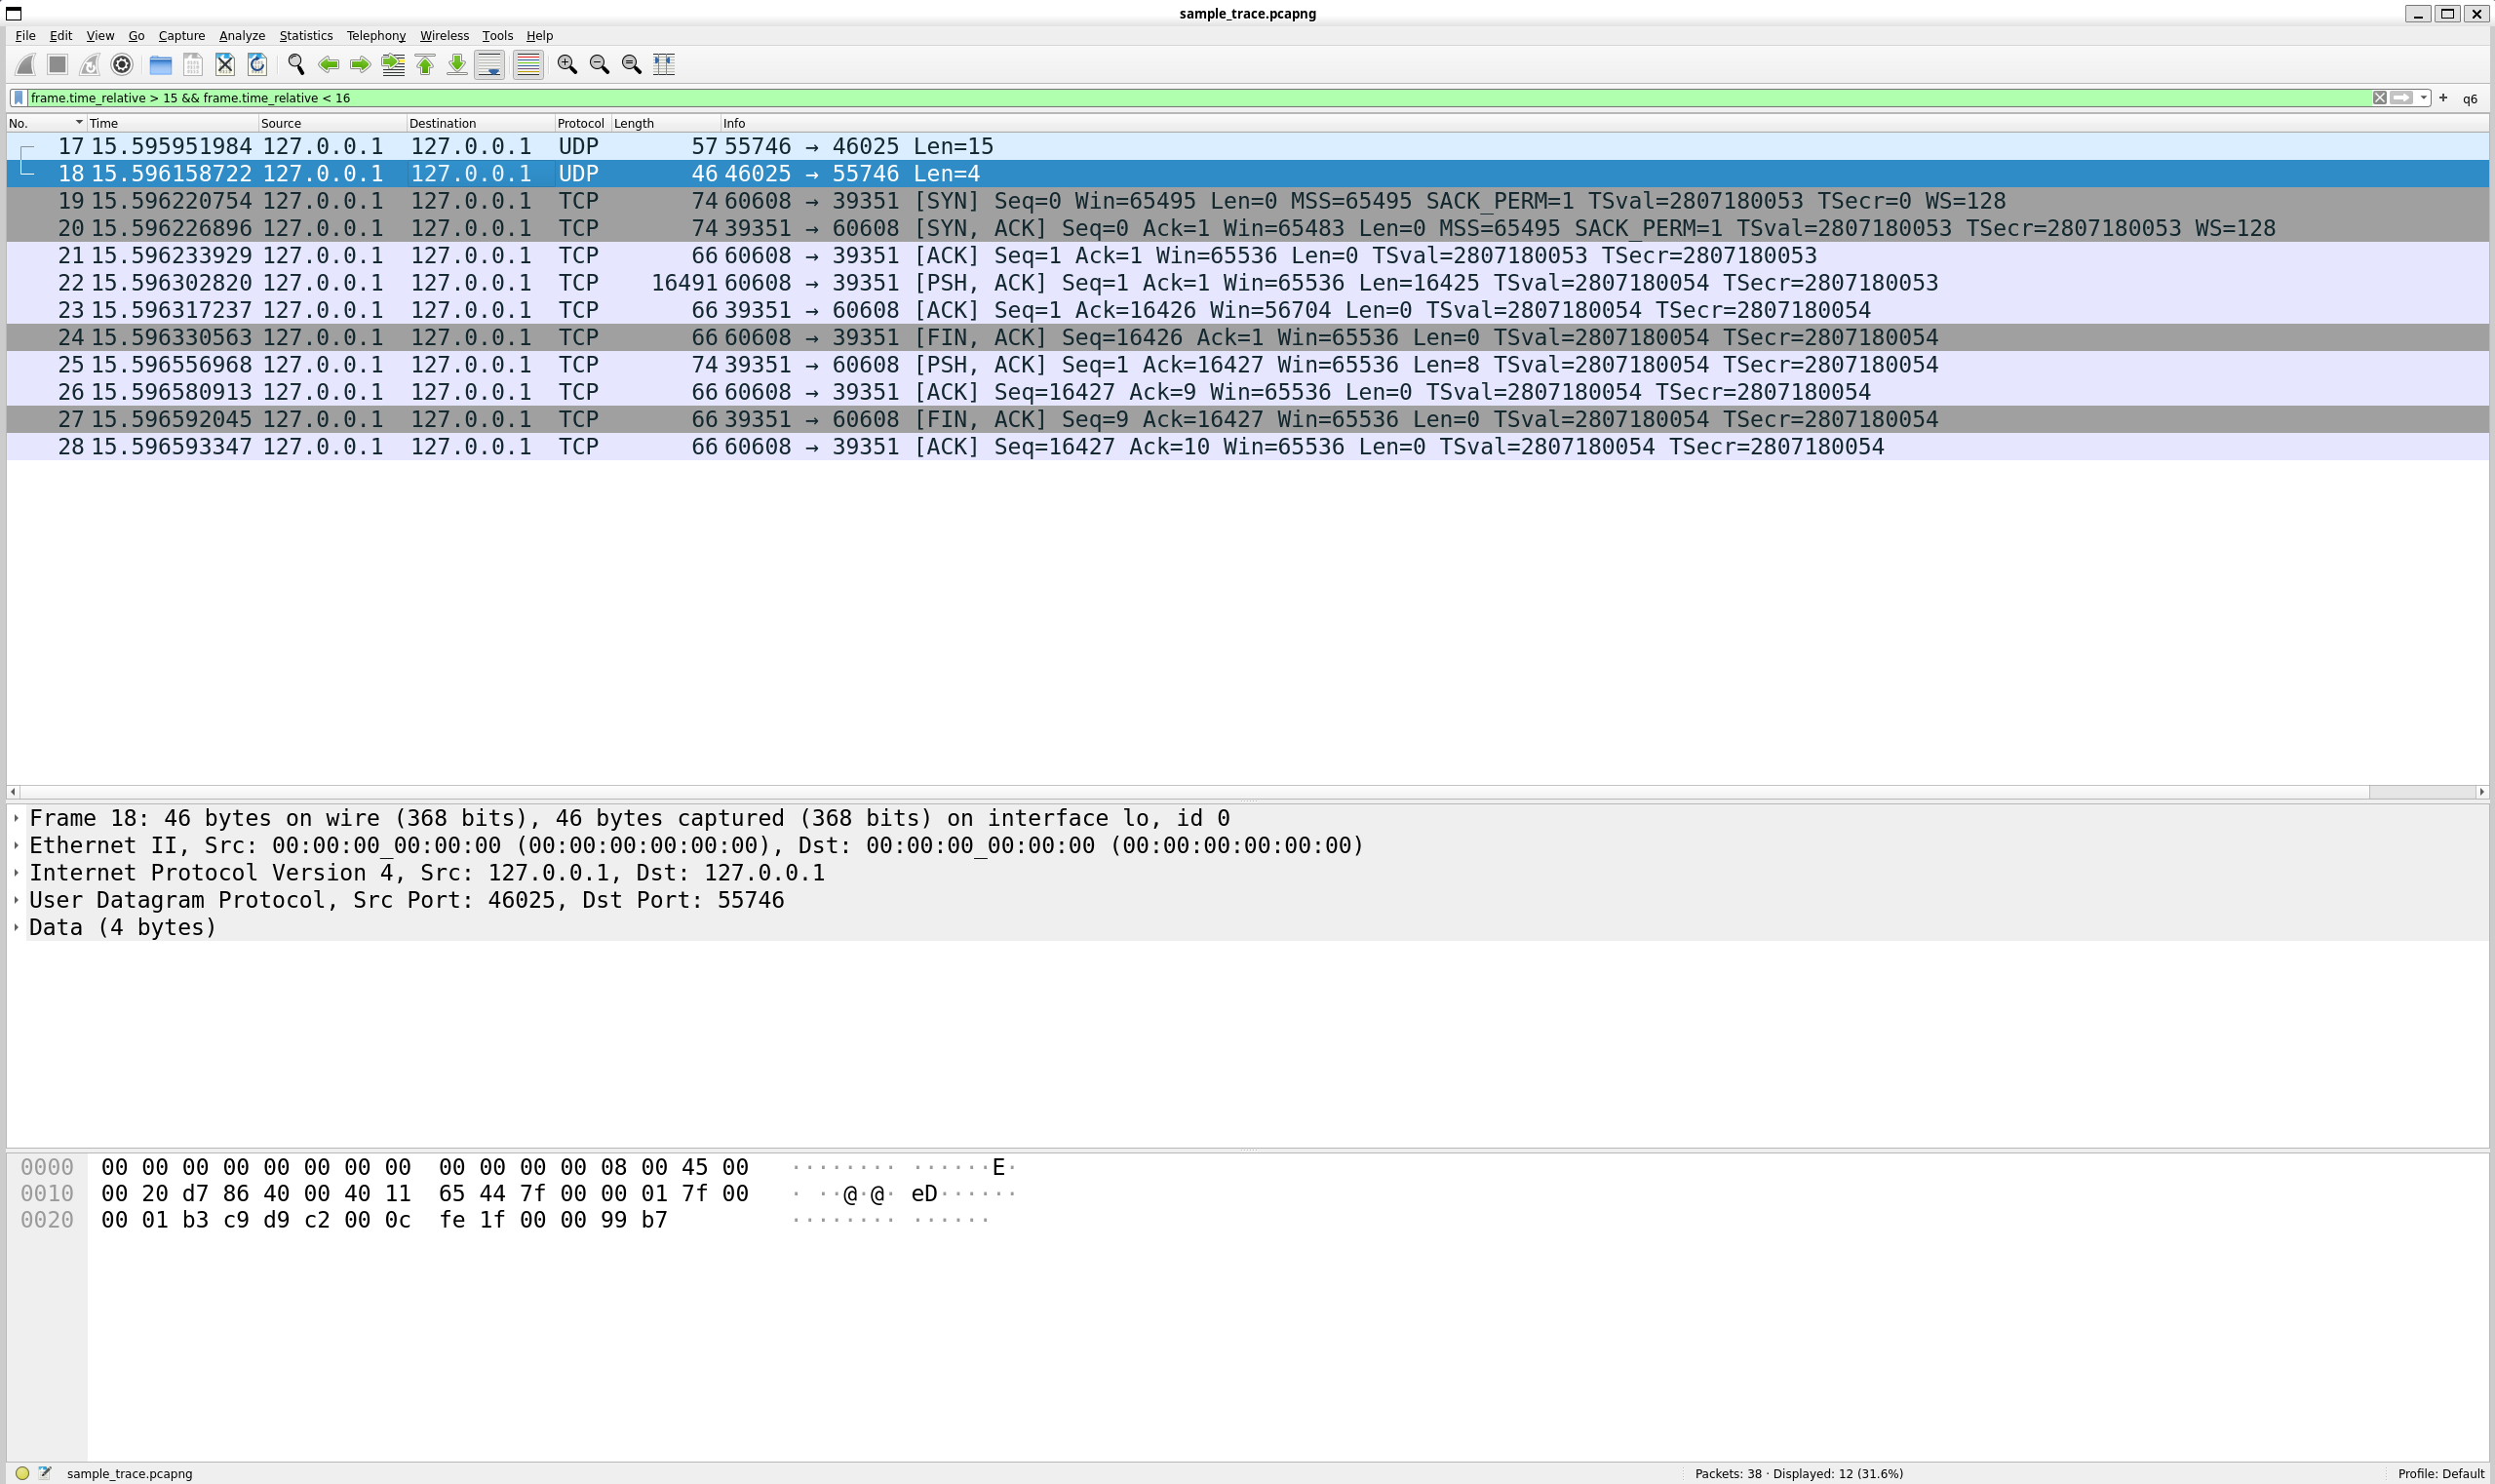
\includegraphics[scale=0.34]{3.3q6.png}
    \end{center}
\end{quote}

\end{document}
